\section{OOD}
\subsection{Ziel des Entwurfs}
  \begin{itemize}[leftmargin=0.5cm]
    \item Spezifizierte Anwendung auf einer Plattform unter den geforderten technischen
      Randbedingungen zu realisieren
    \item Entwurf liegt noch in einem höheren Abstraktionsniveau als in der Implementierung
    \item In der Entwurfsphase wird das OOD-Modell unter den Gesichtspunkten
      der Effizienz und Standardisierung konzipiert.
    \item Jede entworfene Klasse kann direkt implementiert werden
    \item Das OOD-Modell baut auf dem OOA-Modell auf
    \item Die Namen in dem OOD-Modell sollten der Syntax der jeweiligen Programmiersprache
      entsprechen.
  \end{itemize}

  \parbox{9cm}{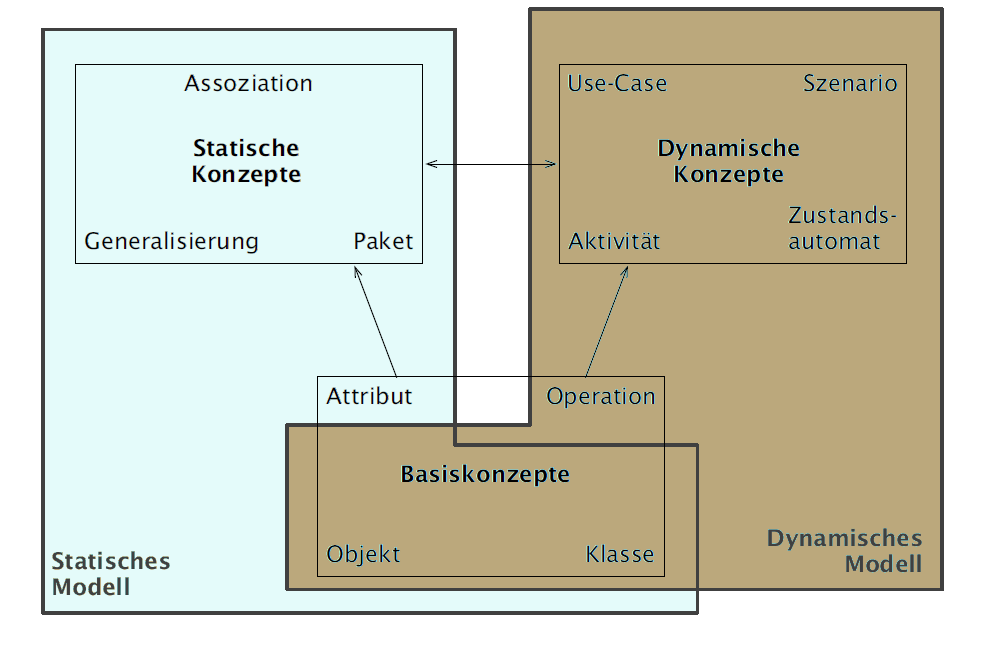
\includegraphics[width=9cm]{./bilder/Konzepte.png}}
  
\subsection{Klassen \balzert{252}}
  \begin{description}
    \item[parametrisierte Klasse]
      Template
    \item[Container Klasse]
      dient zur Verwaltung von einer Menge von Objekten einer anderen Klasse
      (typischerweise als Array implementiert)
    \item[Schnittstelle \Balzert{256}]
      \parbox{5cm}{ähnlich wie abstrakte Klasse, aber \textbf{keine Operation} ist implementiert}
      \hspace{0.5cm}
      \parbox{7cm}{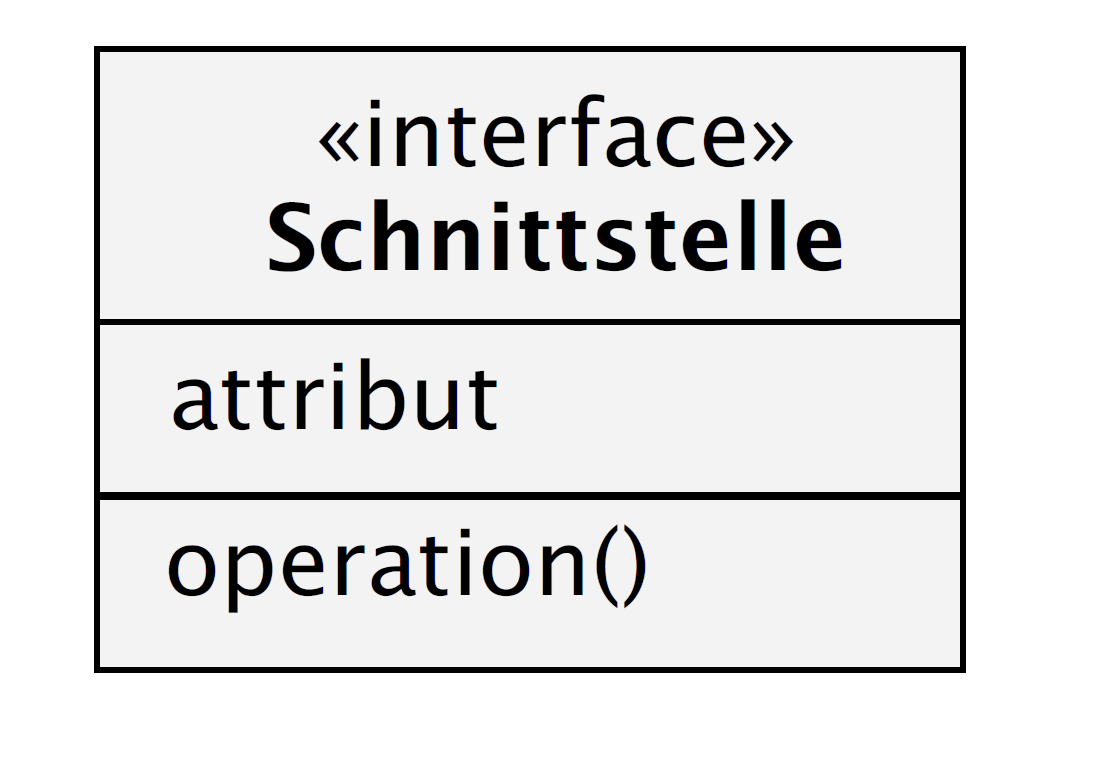
\includegraphics[width=7cm]{./bilder/Schnittstelle.png}}
    \item[Implementierung]
      siehe \Balzert{258, 259}
  \end{description}
  

\subsection{Attribut \balzert{261}}
  \begin{description}
    \item[Sichtbarkeit]
      \begin{itemize}[leftmargin=0.5cm]
        \item[$+$] public
        \item[$\#$] protected
        \item[$-$] privat
        \item[$\sim$] package
      \end{itemize}
    \item[Klassenattribute]
      werden durch \underline{Unterstrichen} gekennzeichnet und mit \textbf{static} implementiert
    \item[Notation]
      Sichtbarkeit / \textbf{name} : Typ [Multiplizität] = Anfangswert $\lbrace$Eigenschaftswert$\rbrace$ \\
    \parbox{6cm}{
      \item[Eigenschaftswerte]
        siehe \Balzert{263}
      \item[Implementation]
        siehe \Balzert{264} }
    \parbox{6cm}{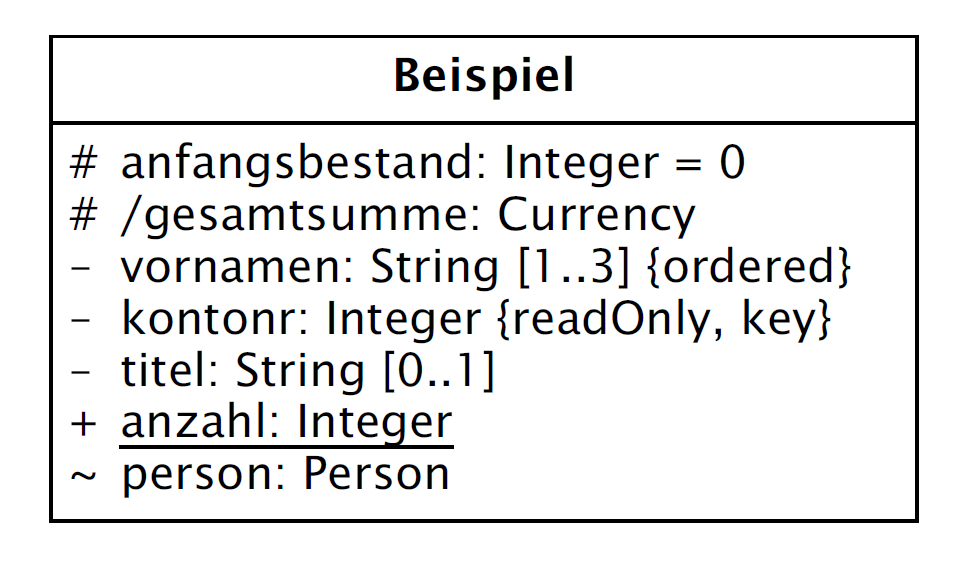
\includegraphics[width=5cm]{./bilder/Notation_Attribute.png}}
  \end{description}
  
  
\subsection{Operationen \balzert{266}}
  \begin{description}
    \item[Notation]
      Sichtbarkeit \textbf{name} (Parameterliste) : Ergenistyp $\lbrace$Eigenschaftswert$\rbrace$
    \item[Parameter]
      Richtung parametername : Typ [Multiplizität] = Anfangswert $\lbrace$Eigenschaftswert$\rbrace$ \\
      \parbox[t]{2cm}{Richtung: }
      \parbox[t]{2cm}{$\bullet$ in \\ $\bullet$ out \\ $\bullet$ inout \\ $\bullet$ return} \\
      siehe \Balzert{267}
    \item[Eigenschaftswerte]
      siehe \Balzert{268}
    \item[Implementation]
      siehe \Balzert{269}
  \end{description}
  
\subsection{Komponente \balzert{273}}
  \begin{minipage}{12cm}
    Eine Komponente ist ein Softwarebaustein, der über klar definierte Schnittstellen, Verhalten bereitstellt.
    Das Innenleben der Komponente bleibt gegen aussen verborgen
  \end{minipage}
  \begin{minipage}{6cm}
    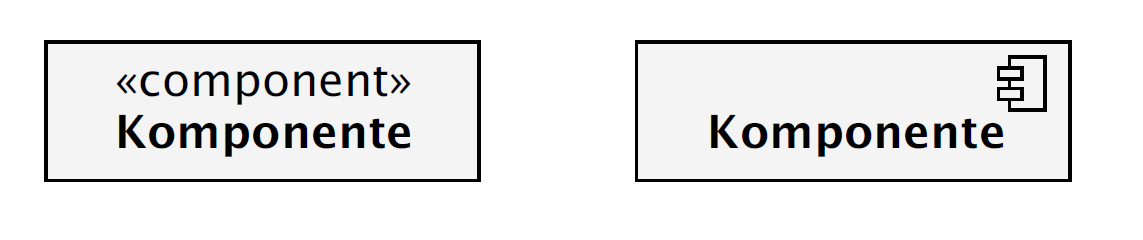
\includegraphics[width=6cm]{./bilder/Komponente.png}
  \end{minipage}
  

\subsection{Assoziation \balzert{284}}
  By-Value wird automatisch mit einer Komposition erstellt.
  \begin{description}[leftmargin=3.5cm]
    \item[Navigierbarkeit]
      \parbox{5cm}{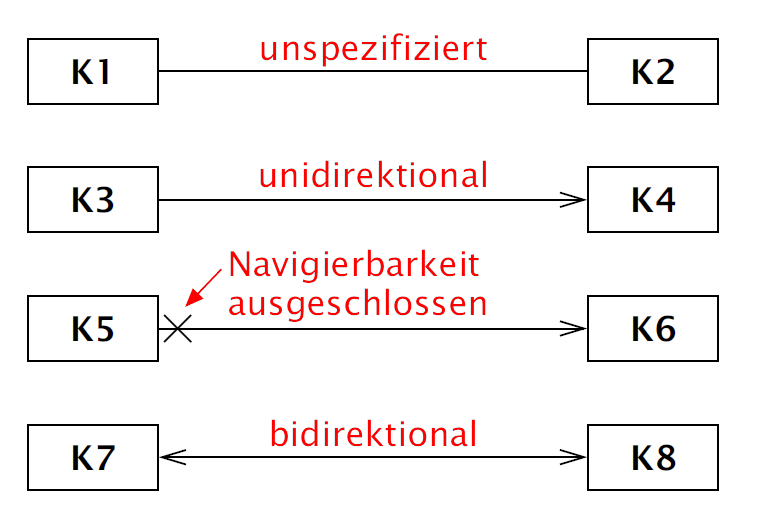
\includegraphics[width=5cm]{./bilder/Navigierbarkeit.png}}
      \hspace{3cm}
      \parbox{8cm}{
      \textbf{Auflösen einer Assoziationsklasse}\\
      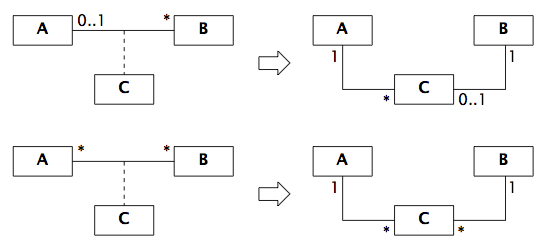
\includegraphics[width = 6cm]{./bilder/Aufloesen_Assoziationsklasse}}
      
    \item[Notation]
      \parbox{8cm}{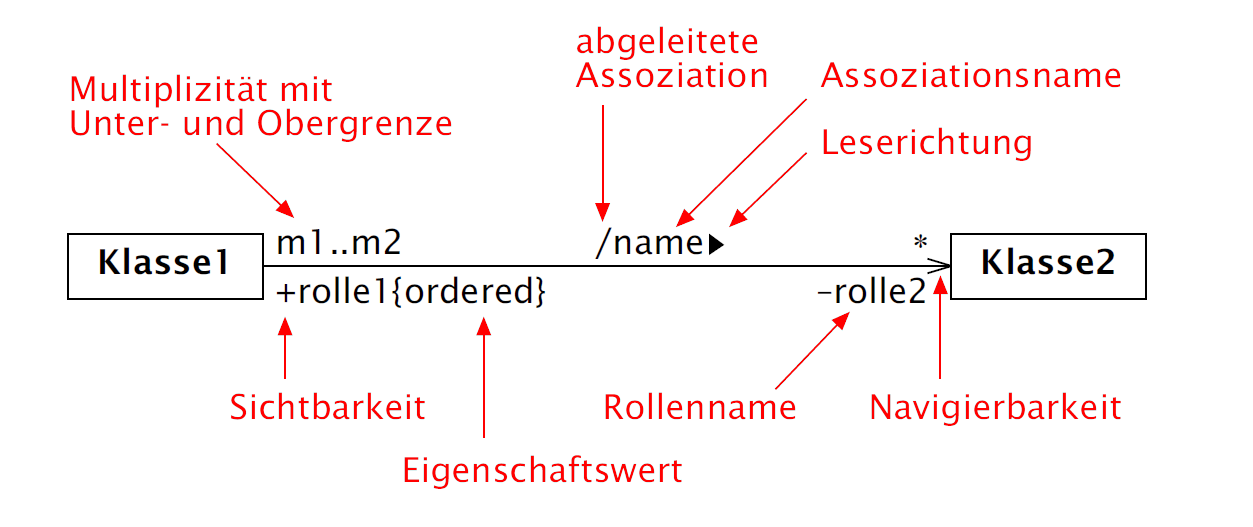
\includegraphics[width=8cm]{./bilder/Notation_Assozi_1.png}}
      \parbox{7cm}{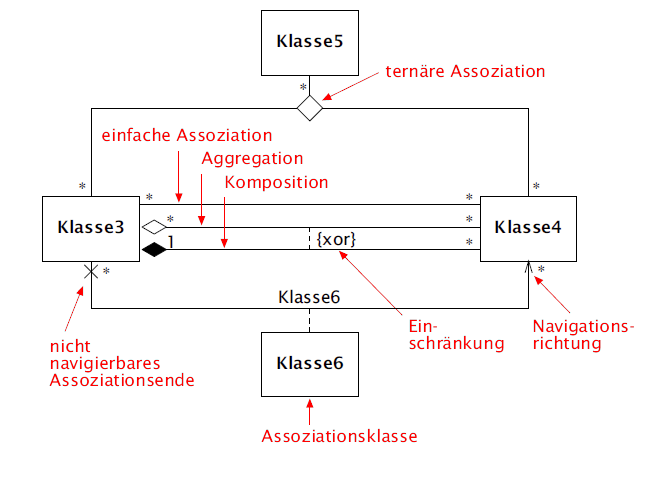
\includegraphics[width=7cm]{./bilder/Notation_Assozi_2.png}}
    \item[Eigenschaftswerte]
      siehe \Balzert{288}
    \item[Implementation]
      siehe \Balzert{291}
  \end{description}

\subsection{Polymorphismus \balzert{293}}
  Polymorphismus ermöglicht es, den gleichen Namen für gleichartige Operationen,
  in verschiedenen Klassen zu gebrauchen.
  \begin{description}
    \item[]
    \item[Notation]
      Operation \textit{kursiv} schreiben
    \item[Deklaration]
      mit \textbf{virtual} deklarieren
    \item[Implementation]
      siehe \Balzert{298}
  \end{description}
  
\subsection{Generalisierung \balzert{300}}
  \begin{description}
    \item[Generalisierungseigenschaften]
      siehe \Balzert{302}
    \item[Notation]
      \parbox{15cm}{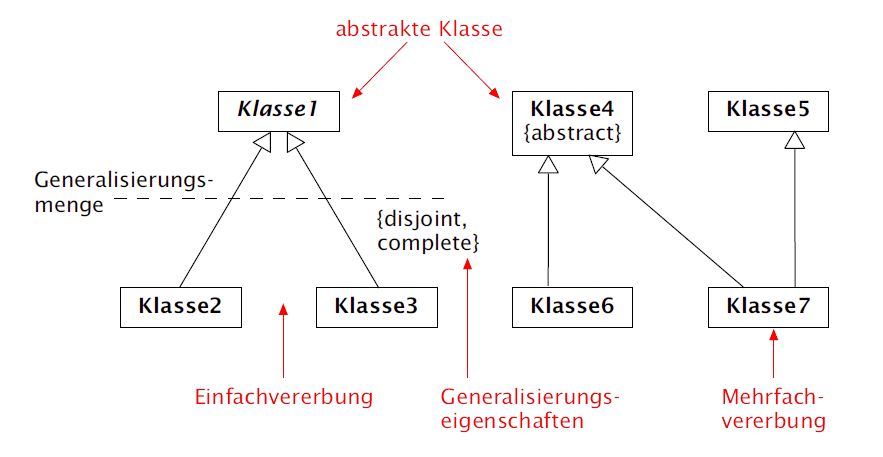
\includegraphics[width=8cm]{./bilder/Notation_Generalisierung.png}}
    \item[Implementation]
      siehe \Balzert{305}
  \end{description}
  

\subsection{Szenario \balzert{327}}
  bezieht sich auf Sequenzdiagramme
  \begin{description}
    \item[synchrone Nachricht]
      Der Sender wartet bis der Empfänger die Verarbeitung komplett durchgeführt hat.
    \item[asynchrone Nachricht]
      Der Sender wartet \textbf{nicht} bis auf den Empfänger, sondern setzt seine Verarbeitung
      parallel fort.
    \item[kominierte Fragmente]
      siehe \Balzert{331}
    \item[Notation]
      \parbox{15cm}{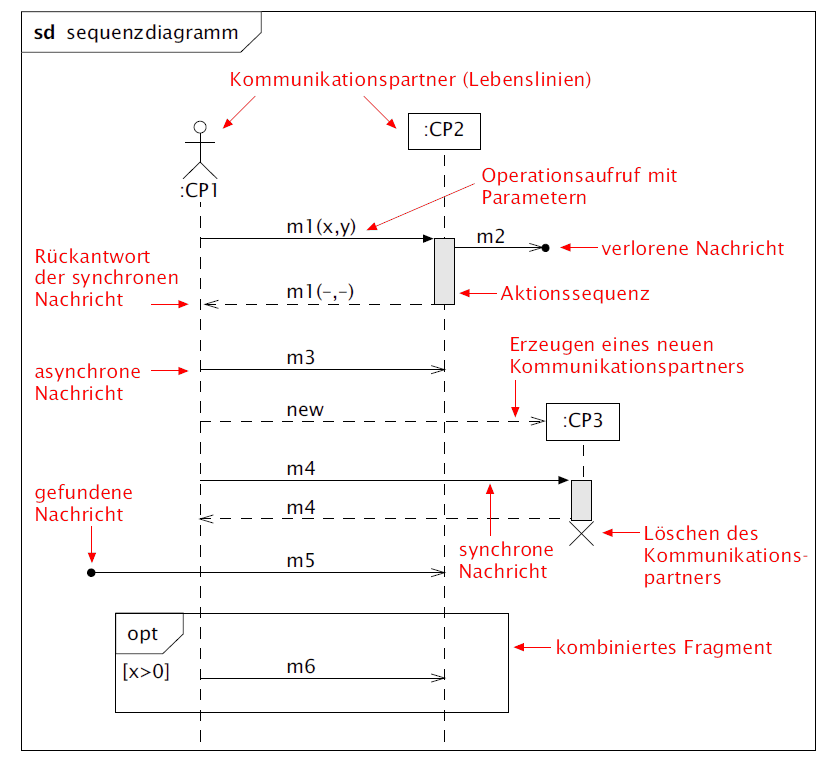
\includegraphics[width=10cm]{./bilder/Notation_Sequanzdia.png}}
  \end{description}
  
\subsection{Entwurfsmuster \balzert{355}}